\subsection{Outline}

Ola is a full stack developer framework for zero-knowledge applications, the whole framework is shown as figture\ref{fig:Ola framework}:
\begin{figure}[!ht]
    \centering
    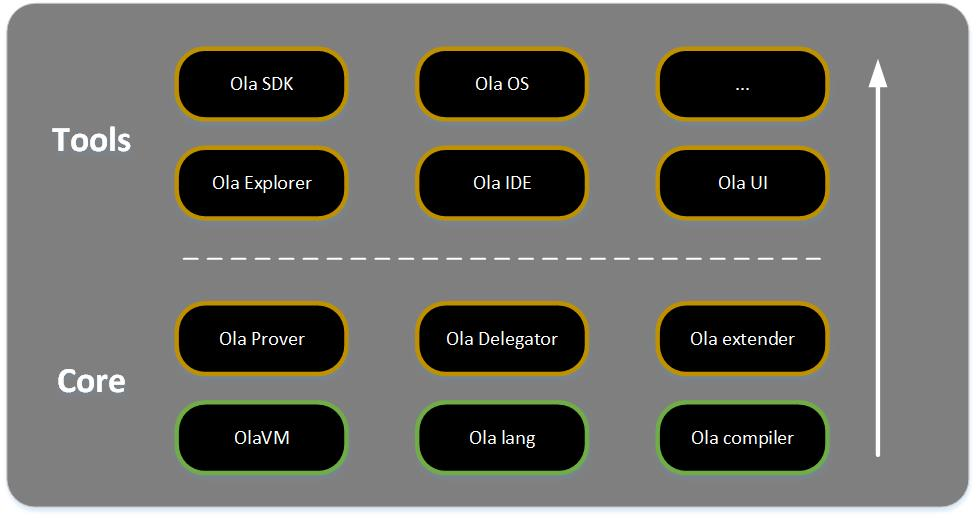
\includegraphics[width=0.6\textwidth]{vm/Ola framework.jpg}
    \caption{Ola framework}
    \label{fig:Ola framework}
\end{figure}

The green wires stands for the modules we have implemented, and others stand for the modules we will implement in the future. In the remaining sections of this whitepaper, we will introduce those modules 
as follows:
\begin{itemize}
    \item Section \ref{sec:olavm-a-full-featured-zk-friendly-zkvm} mainly describes the design of the virtual machine of OlaVM, include all tricks to get zk-friendly;
    \item Section \ref{sec:ola-lang} mainly describes the design of customize SM language, Ola-lang and the framework of Ola complier based LLVM;
    \item Section \ref{sec:ola-compiler} mainly describes the design of Ola compiler;
    \item Section \ref{sec:zk-zkvm} mainly describes some key points to get privacy;
    \item Section \ref{sec:algorithms} mainly describes the algorithms used in Ola, include the zk arround and hardware acceleration algorithms;
    \item Section \ref{section:appendix} mainly describes the key features supported in the future and the frameworks;
\end{itemize}